

\section{Evaluation}\label{sec:eval}

\stitle{Experimental settings}. We start with experimental settings.

\etitle{Datasets and Queries}.

\begin{figure*}[tb!]
  \vspace{-1.7ex}
  \begin{center}
    \begin{minipage}[t]{\textwidth}

      \begin{subfigure}[b]{0.24\textwidth}
        \includegraphics[width=\textwidth]{exp/blank.eps}
        \caption{Scalability (vary thread count)}
        \label{fig:scale-thread}
      \end{subfigure}
      \vspace{.4em}
      \hfill
      \begin{subfigure}[b]{0.24\textwidth}
        \includegraphics[width=\textwidth]{exp/blank.eps}
        \caption{Scalability (vary scale factor)}
        \label{fig:scale-graph}
      \end{subfigure}
      \hfill
      \begin{subfigure}[b]{0.24\textwidth}
        \includegraphics[width=\textwidth]{exp/blank.eps}
        \caption{End-to-end evaluation (\ldbc)}
        \label{fig:e2e-ldbc}
      \end{subfigure}
      \hfill
      \begin{subfigure}[b]{0.24\textwidth}
        \includegraphics[width=\textwidth]{exp/blank.eps}
        \caption{End-to-end evaluation (\imdb)}
        \label{fig:e2e-imdb}
      \end{subfigure}


            \begin{subfigure}[b]{0.24\textwidth}
        \includegraphics[width=\textwidth]{exp/blank.eps}
        \caption{Scalability (vary thread count)}
        \label{fig:scale-thread}
      \end{subfigure}
      \vspace{.4em}
      \hfill
      \begin{subfigure}[b]{0.24\textwidth}
        \includegraphics[width=\textwidth]{exp/blank.eps}
        \caption{Scalability (vary scale factor)}
        \label{fig:scale-graph}
      \end{subfigure}
      \hfill
      \begin{subfigure}[b]{0.24\textwidth}
        \includegraphics[width=\textwidth]{exp/blank.eps}
        \caption{End-to-end evaluation (\ldbc)}
        \label{fig:e2e-ldbc}
      \end{subfigure}
      \hfill
      \begin{subfigure}[b]{0.24\textwidth}
        \includegraphics[width=\textwidth]{exp/blank.eps}
        \caption{End-to-end evaluation (\imdb)}
        \label{fig:e2e-imdb}
      \end{subfigure}

            \begin{subfigure}[b]{0.24\textwidth}
        \includegraphics[width=\textwidth]{exp/blank.eps}
        \caption{Scalability (vary thread count)}
        \label{fig:scale-thread}
      \end{subfigure}
      \vspace{.4em}
      \hfill
      \begin{subfigure}[b]{0.24\textwidth}
        \includegraphics[width=\textwidth]{exp/blank.eps}
        \caption{Scalability (vary scale factor)}
        \label{fig:scale-graph}
      \end{subfigure}
      \hfill
      \begin{subfigure}[b]{0.24\textwidth}
        \includegraphics[width=\textwidth]{exp/blank.eps}
        \caption{End-to-end evaluation (\ldbc)}
        \label{fig:e2e-ldbc}
      \end{subfigure}
      \hfill
      \begin{subfigure}[b]{0.24\textwidth}
        \includegraphics[width=\textwidth]{exp/blank.eps}
        \caption{End-to-end evaluation (\imdb)}
        \label{fig:e2e-imdb}
      \end{subfigure}

            \begin{subfigure}[b]{0.24\textwidth}
        \includegraphics[width=\textwidth]{exp/blank.eps}
        \caption{Scalability (vary thread count)}
        \label{fig:scale-thread}
      \end{subfigure}
      \vspace{.4em}
      \hfill
      \begin{subfigure}[b]{0.24\textwidth}
        \includegraphics[width=\textwidth]{exp/blank.eps}
        \caption{Scalability (vary scale factor)}
        \label{fig:scale-graph}
      \end{subfigure}
      \hfill
      \begin{subfigure}[b]{0.24\textwidth}
        \includegraphics[width=\textwidth]{exp/blank.eps}
        \caption{End-to-end evaluation (\ldbc)}
        \label{fig:e2e-ldbc}
      \end{subfigure}
      \hfill
      \begin{subfigure}[b]{0.24\textwidth}
        \includegraphics[width=\textwidth]{exp/blank.eps}
        \caption{End-to-end evaluation (\imdb)}
        \label{fig:e2e-imdb}
      \end{subfigure}
    \end{minipage}
  \end{center}
  \vspace{-3.4ex}
  \caption{Performance Evaluation}
  \vspace{-1.7ex}
  \label{fig:eval}
\end{figure*}

\etitle{Environment}.

\vspace{-.3em}
\stitle{Exp-1: Estimation Accuracy}.

\stitle{Exp-2: Estimation Latency}.

\stitle{Exp-3: PDS Construction Latency}.

\stitle{Exp-4: PDS Maintenance Efficiency}.

\stitle{Exp-5: Scalability of DS Construction}.

\stitle{Exp-6: Micro Benchmarks}.


\stitle{Exp-6: Impact On End-to-End Performance}.